\chapter{Estado del Arte}\label{chapter03}

La predicción de demanda en comercios que operan con productos perecederos representa un desafío significativo debido a la naturaleza volátil y sensible al tiempo de estos bienes. En las últimas décadas, el avance de las tecnologías de inteligencia artificial y aprendizaje automático ha permitido desarrollar soluciones cada vez más sofisticadas para anticipar patrones de consumo y optimizar la producción, con el objetivo de minimizar pérdidas y mejorar la eficiencia operativa.

Este estado del arte presenta una revisión crítica de las soluciones tecnológicas existentes y los enfoques académicos más relevantes aplicados a la predicción de demanda en el sector alimentario, con especial énfasis en productos frescos y perecederos. Se analizan modelos, métricas y tecnologías empleadas, así como las limitaciones que enfrentan estas soluciones, especialmente en contextos de pequeñas y medianas empresas con restricciones operativas y tecnológicas.

A partir de este análisis, se evidencian las oportunidades y necesidades no cubiertas que motivan el desarrollo de la propuesta de este proyecto, orientada a un contexto local con condiciones económicas y sociales específicas, buscando ofrecer una herramienta accesible, flexible y efectiva para comercios minoristas.

\section{Soluciones Tecnológicas Existentes}

En el mercado global existen diversas soluciones tecnológicas orientadas a la predicción de demanda, particularmente en retail alimentario:

\begin{itemize}
    \item \textbf{SAP Forecasting and Replenishment (F\&R)}: Es una herramienta empresarial enfocada en la planificación de inventarios y la reposición automática. Utiliza modelos estadísticos y reglas de negocio, pero no incluye inteligencia artificial. Para eso, SAP ofrece otra solución aparte llamada, \textit{SAP Predictive Replenishment}, orientada a clientes con mayores requerimientos tecnológicos.
    
    \item \textbf{Oracle Retail Demand Forecasting}: Permite hacer pronósticos utilizando algoritmos de aprendizaje automático y tiene en cuenta factores como estacionalidad, promociones o eventos. Es una solución muy completa, pero está pensada para grandes empresas y requiere una inversión importante para su implementación, lo que la hace poco viable para PYMEs.
    
    \item \textbf{BakePlan}: Es una herramienta pensada específicamente para panaderías, especialmente en Europa. Estima la cantidad ideal de productos horneados por día basándose en ventas pasadas y condiciones climáticas. Si bien logra buenos resultados en reducción de merma, su aplicación está limitada a contextos muy estructurados, y no se adapta fácilmente a entornos informales o menos digitalizados.
    
    \item \textbf{Blue Yonder Luminate}: es una plataforma en la nube que utiliza inteligencia artificial para realizar predicciones de demanda. Está dirigida principalmente a grandes cadenas y supermercados, pero no es una opción adecuada para pequeños comercios, ya que requiere cierto grado de digitalización previa y personal técnico capacitado para su uso.
\end{itemize}

Estos estudios confirman que los modelos neuronales como LSTM y Bi-LSTM superan en precisión a los enfoques clásicos, especialmente en entornos con múltiples variables externas (como el clima), lo que refuerza su aplicabilidad en el presente proyecto.

\section{Estudios y enfoques académicos}

Investigaciones recientes han abordado la predicción de demanda para alimentos perecederos con distintos enfoques:

\begin{itemize}
    \item Se han comparado distintos modelos de \textit{machine learning} para la predicción de demanda en la industria alimentaria, como Random Forest, SVM y LSTM. En estas pruebas, el modelo LSTM fue el que logró el menor error promedio (RMSE), al demostrar una mejor capacidad para capturar patrones temporales no lineales \parencite{nassibi2023}.

    \item En el ámbito del \textit{e-commerce} de alimentos frescos, se ha utilizado un modelo Bi-LSTM para predecir la demanda logística. Al incorporar variables climáticas y festivos, se logró reducir el MAE en un 12{,}6\,\% respecto de los modelos base \parencite{ni2022}.

    \item También se ha propuesto el modelo LSTM-MSNet para predecir múltiples series temporales con patrones estacionales. Este enfoque superó a modelos tradicionales como Prophet y Holt-Winters, especialmente en escenarios con datos ruidosos o incompletos \parencite{bandara2020}.
\end{itemize}

Estos estudios confirman que los modelos neuronales como LSTM y Bi-LSTM superan en precisión a los enfoques clásicos, especialmente en entornos con múltiples variables externas (como el clima), lo que refuerza su aplicabilidad en el presente proyecto.



\begin{table}[t]
    \centering
    \renewcommand{\arraystretch}{1.3}
    \caption{Comparación de enfoques}
    \label{tab:comparacion}
    \begin{tabular}{|p{2.9cm}|p{2cm}|p{3cm}|p{5cm}|}
        \hline
        \textbf{Solución} & \textbf{Tipo} & \textbf{Tecnologías principales} & \textbf{Limitaciones destacadas} \\
        \hline
        SAP F\&R & Comercial & ARIMA, reglas heurísticas & Costoso, complejo \\
        \hline
        Oracle RDF & Comercial & ML + estacionalidad & Requiere datos limpios (MAPE, RMSE) \\
        \hline
        BakePlan & Comercial (PYME) & Reglas, regresiones & No escalable (\% de merma) \\
        \hline
        Nassibi et al. (2023) & Académico & LSTM, Random Forest & No adaptado a Argentina (MAE, RMSE) \\
        \hline
        Ni et al. (2022) & Académico & Bi-LSTM & Datos estructurados (MAE, RMSE) \\
        \hline
        Propuesta actual (PFI) & Académico & LSTM, Prophet, LLMs & Datos limitados iniciales (MAE, RMSE, MAPE) \\
        \hline
    \end{tabular}
\end{table}


\section{Aporte diferencial del proyecto}

El sistema propuesto en este proyecto se distingue de las soluciones analizadas por las siguientes características:

\begin{itemize}
    \item \textbf{Accesibilidad}: pensado específicamente para pequeños comercios argentinos sin sistemas previos de gestión ni personal técnico.

    \item \textbf{Multimodalidad}: permite la carga de registros mediante imágenes, utilizando modelos OCR y LLMs, lo cual no está presente en las herramientas comerciales revisadas.

    \item \textbf{Interfaz natural}: reemplaza los paneles tradicionales por un chatbot conversacional en lenguaje natural, facilitando el uso incluso por usuarios no técnicos.

    \item \textbf{Orientación local}: los modelos se entrenan considerando variables específicas como clima y feriados de Buenos Aires en el año 2025.
\end{itemize}


\section{User Research}

Para validar la propuesta y diseñar una herramienta que responda a problemáticas reales del entorno operativo, se llevó a cabo una instancia de investigación cualitativa centrada en usuarios representativos del mercado objetivo. La metodología consistió en entrevistas semi-estructuradas a actores clave del rubro de productos perecederos, con el objetivo de identificar necesidades, limitaciones tecnológicas actuales, y oportunidades de mejora en los procesos de planificación y producción diaria. A continuación, se expone la información más significativa relevada durante las entrevistas.

\subsection{Entrevista a Bruno, dueño de la Confitería ``Salvador''}

Con el objetivo de comprender de manera más profunda el contexto operativo de los pequeños comercios de productos perecederos, se entrevistó a Bruno, propietario de la confitería ``Salvador'', un negocio con más de 20 años de trayectoria en la ciudad. Esta entrevista buscó obtener información cualitativa para validar el desarrollo de una herramienta de predicción de demanda y conocer el grado de adopción tecnológica actual.

La confitería Salvador se especializa en la venta de café y postres, y emplea a más de 10 personas. Bruno señaló que el café y productos relacionados son los más demandados, mientras que los postres presentan una menor rotación. Según indicó, los productos tienen una duración estimada de un día en inventario, lo que evidencia una rotación diaria muy alta y la necesidad de una planificación precisa.

Respecto a la gestión operativa, cada local es responsable de su propia reposición de productos. La producción diaria se define en función de los faltantes observados y de estimaciones realizadas a partir del comportamiento histórico de ventas. Entre los factores considerados para estas estimaciones, se destacó la influencia de los fines de semana, dado que la demanda suele incrementarse en esos días.

Bruno remarcó que la precisión en la estimación de la demanda es muy importante para el negocio, ya que permite evitar tanto el quiebre de stock como la sobreproducción. Si bien actualmente el desperdicio no representa un problema crítico, sí es una preocupación constante por sus implicancias en los costos y la eficiencia operativa.

En cuanto a la tecnología utilizada, la confitería ya emplea el sistema Maxirest para la gestión de inventario. Sin embargo, Bruno manifestó su disposición a adoptar nuevas herramientas siempre que aporten mejoras tangibles, como la reducción de desperdicios o el incremento de ventas.

Particularmente, se mostró interesado en una herramienta que permita predecir la demanda de forma más precisa incorporando datos históricos, variables climáticas y otros factores externos. Considera que una solución de este tipo le permitiría ajustar la producción diaria de manera más eficiente, reducir mermas y mejorar la toma de decisiones operativas.

Este testimonio pone de manifiesto la necesidad de soluciones accesibles, basadas en inteligencia artificial, que puedan integrarse fácilmente en los procesos de pequeños comercios. Además, valida el enfoque propuesto por este proyecto, que busca dotar a estos actores de herramientas tecnológicas que mejoren la eficiencia y la sustentabilidad de sus operaciones.


\subsection{Entrevista a María, dueña de ``Tiendas Naturales''}

Con el objetivo de comprender mejor las dinámicas operativas y los desafíos específicos de los comercios que gestionan productos perecederos, se entrevistó a María, propietaria de Tiendas Naturales, un negocio especializado en ofrecer productos saludables y menús ejecutivos. Esta entrevista tiene como propósito validar la efectividad de una herramienta de predicción de demanda diseñada para optimizar la producción y reducir el desperdicio de productos perecederos en comercios de características similares.

Tiendas Naturales ha estado en funcionamiento durante 15 años y cuenta con un equipo comprometido de más de 10 empleados. Este establecimiento se especializa en ofrecer una variedad de productos saludables, que incluyen desde menús ejecutivos hasta opciones para meriendas y productos más ligeros para quienes buscan alternativas saludables a lo largo del día. Los menús ejecutivos son su producto principal, dada la alta demanda, aunque también comercializan jugos naturales, ensaladas y repostería saludable como parte de su oferta de meriendas.

\indent A pesar de que las meriendas tienen una menor rotación, representan una parte importante de la oferta, especialmente en horas de la tarde. Los productos en inventario permanecen, en promedio, entre dos a tres días, lo que refleja una alta rotación. Esta dinámica permite mantener una oferta fresca y de calidad, aunque plantea el reto constante de prever con precisión la demanda para evitar pérdidas por sobreproducción o quiebres de stock.

\indent María explicó que actualmente el manejo de inventarios no está automatizado, ya que no disponen de un sistema formal de gestión. La estimación de cantidades a producir o adquirir se basa mayormente en un análisis manual de las ventas pasadas. Este proceso depende del criterio y la experiencia del equipo, sin incorporar herramientas tecnológicas que integren variables externas como el clima o eventos especiales.

\indent Este enfoque, si bien funcional en la práctica, presenta limitaciones frente a escenarios de alta variabilidad en la demanda. La ausencia de un sistema predictivo dificulta la anticipación a días de mayor demanda y eleva el riesgo de errores en la planificación. Aunque la experiencia del equipo permite mantener cierta regularidad, María reconoció que una herramienta más precisa y dinámica sería muy beneficiosa para mejorar la eficiencia operativa.

\indent En la actualidad, la planificación de la producción se realiza observando las ventas anteriores y ajustando de acuerdo con patrones repetidos. No obstante, María destacó la necesidad de incorporar factores adicionales, como promociones, festividades o eventos locales, que pueden impactar significativamente en la demanda de ciertos productos.

\indent En cuanto al desperdicio, si bien no es un problema crítico, la empresa experimenta en ocasiones pérdidas por productos que no logran venderse a tiempo. Esto ocurre principalmente con jugos y postres, los cuales presentan un alto nivel de obsolescencia debido a su vida útil muy corta. Cada pérdida representa un impacto económico y operativo, subrayando la importancia de una mejor gestión preventiva basada en datos.

\indent El negocio actualmente emplea un software de gastronomía que brinda funcionalidades básicas de control de inventario y ventas, pero no incorpora capacidades predictivas. María expresó que, si existiera una herramienta que permita reducir desperdicios y mejorar ventas mediante una estimación más precisa de la demanda, estaría dispuesta a adoptarla sin inconvenientes. Esta actitud positiva demuestra una clara apertura a la innovación tecnológica por parte del negocio.

\indent Finalmente, al ser consultada sobre su interés en soluciones basadas en IA, María manifestó entusiasmo por contar con una herramienta que prediga la demanda usando datos históricos, condiciones climáticas y eventos externos. Según afirmó, esto le permitiría ajustar la producción a la demanda real, minimizar mermas, reducir costos operativos y mejorar la disponibilidad de productos en momentos clave.

\indent En resumen, la entrevista a María refuerza la necesidad de soluciones tecnológicas accesibles y adaptables para la predicción de demanda en pequeños comercios, y valida el enfoque adoptado por este proyecto como una herramienta de mejora para la sostenibilidad y eficiencia operativa del sector.


\subsection{Conclusión del User Research}

\indent El relevamiento realizado a través de entrevistas a dueños de comercios que operan con productos perecederos permitió identificar con claridad necesidades concretas y limitaciones actuales en la gestión de la demanda, el inventario y la producción diaria. Si bien ambos entrevistados demostraron tener experiencia en la operación de sus negocios y, en algunos casos, el uso de herramientas básicas de gestión, se evidenció la ausencia de sistemas predictivos avanzados capaces de integrar variables externas (como clima, eventos o estacionalidad) en la planificación de la producción.

\indent Asimismo, surgió un interés genuino en adoptar soluciones tecnológicas que permitan reducir el desperdicio, mejorar la eficiencia operativa y optimizar la toma de decisiones. Ambos entrevistados expresaron que una herramienta de predicción de demanda, basada en IA y alimentada por datos históricos y contextuales, sería útil y bienvenida en sus negocios, siempre que su adopción sea accesible y su impacto tangible.

\indent Los hallazgos obtenidos validan el enfoque del presente proyecto, al confirmar la existencia de un problema no resuelto y una oportunidad concreta de mejora mediante la incorporación de tecnología. La información recopilada durante esta etapa de investigación será insumo clave para el diseño funcional de la herramienta, su adecuación al entorno real y su potencial adopción por parte del mercado objetivo.

\newpage % <-- salto de página



\begin{figure}[h]
    \centering
    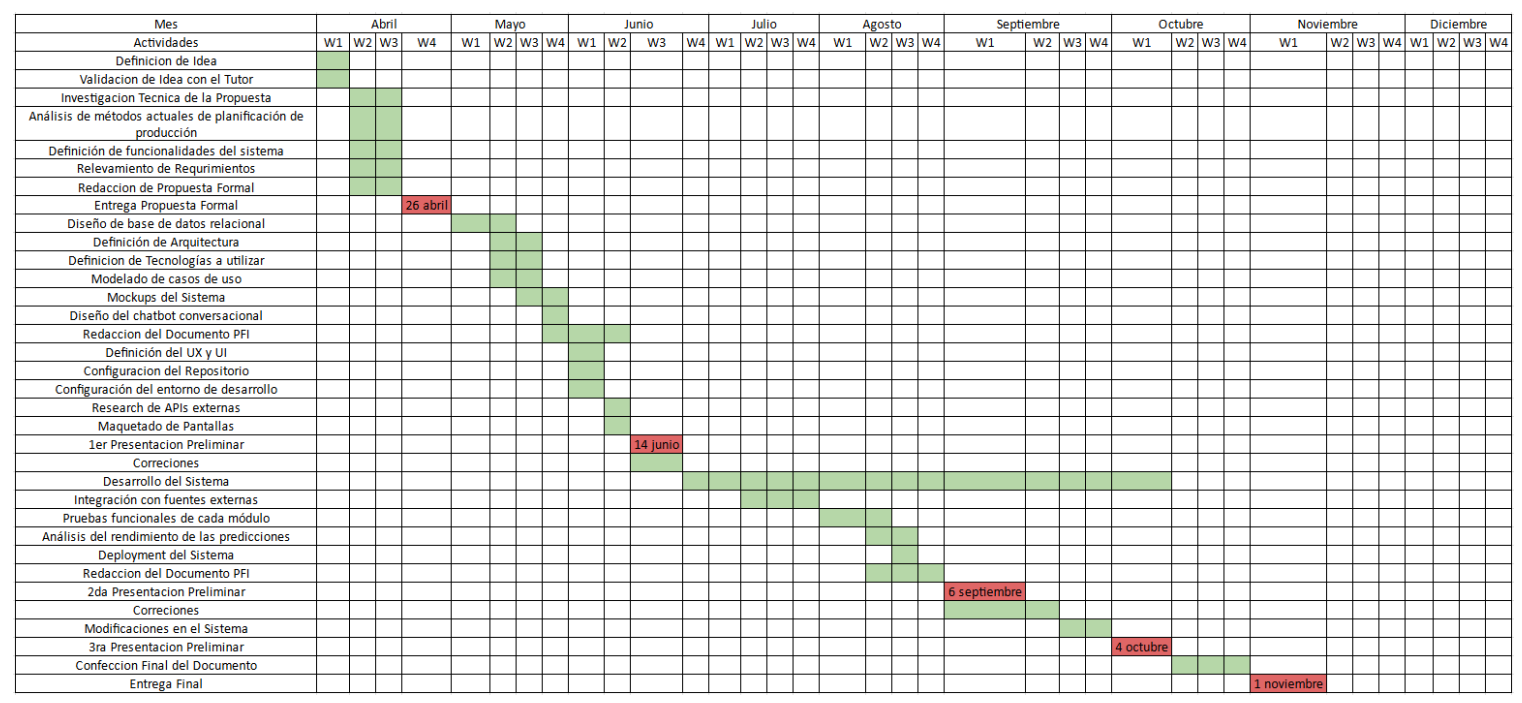
\includegraphics[width=0.7\textwidth]{images/cronograma.png}
    \caption{Cronograma de Actividades}
    \label{fig:cronograma}
\end{figure}
